\documentclass[a4paper,12pt]{article} 

\usepackage[top = 2.5cm, bottom = 2.5cm, left = 2.5cm, right = 2.5cm]{geometry} 

\usepackage[T1]{fontenc}
\usepackage[utf8]{inputenc}
\usepackage{amsmath}
\usepackage{multirow}
\usepackage{booktabs} 
\usepackage{tikz}
\usepackage{graphicx} 
\usepackage{amssymb} 
\usepackage{pdfpages}

\usepackage{setspace}
\setlength{\parindent}{0in}

\usepackage{float}

\usepackage{fancyhdr}
\usepackage{enumerate}

\pagestyle{fancy} 
\fancyhf{}
\lhead{\footnotesize PR \& ML: Blatt 2}
\rhead{\footnotesize F. Freter, E. Kirchberger, S. Symhoven \& J. Wustl} %<---- Fill in your lastnames.

\cfoot{\footnotesize \thepage} 

\begin{document}

\thispagestyle{empty} 

\begin{tabular}{p{15.5cm}} 
{\large \bf Pattern Recognition und Machine Learning} \\
Hochschule München \\ Sommersemester 2023  \\ Prof. Dr.-Ing. Claudius Schnörr \\
\hline 
\\
\end{tabular} 

\vspace*{0.3cm} 

\begin{center} 
	{\Large \bf Blatt 2} 
	\vspace{2mm}
	

	{\bf F. Freter, E. Kirchberger, S. Symhoven \& J. Wustl} 
		
\end{center}  

\vspace{0.4cm}

\section*{Aufgabe 1: Bayes-Klassifikator}


\begin{enumerate}[1.)]

	\item 
	
	\begin{align*}
		P(w_1) &= \frac{3000}{3000+2000} = 0,6 \\
		P(w_2) &= \frac{2000}{3000+2000} = 0,4
	\end{align*}

	\item Vorüberlegungen:
	
	Bayes-Formel (A posteriori-Wahrscheinlichkeiten):
	\begin{align*}
		P(w_1 | x) &= \frac{P(x | w_1) * P(w_1)}{P(x)} \\
		P(w_2 | x) &= \frac{P(x | w_2) * P(w_2)}{P(x)}, \\
	\end{align*}

	und die Verbundwahrscheinlichkeit der Ereignisse: 

	\begin{align*}
		P(x) =  P(x|w_1) * P(w_1) + P(x|w_2) * P(w_2)\\
	\end{align*}

	Der Bayes-Klassifikator folgt dann als:

	\begin{align*}
		g^* =  \begin{cases}
			1 & \text{wenn } P(w_1|x) \geq P(w_2|x) \\
		    2 & \text{wenn } P(w_1|x) < P(w_2|x)
		\end{cases} 
	\end{align*}

	Aus den klassenbedingten Wahrscheinlichkeiten kann nun die optimale Klassifizierung 
	anhand des MAP Kriteriums getroffen werden:

	\begin{align*}
		P(x = 1) &= \frac{1}{6} * 0,6 = 0,1 \\
		P(x \in \{2,3,4,5\}) &= \frac{1}{6} * 0,6 + \frac{1}{6} * 0,4 = \frac{1}{6} \\
		P(x = 6) &= \frac{1}{6} * 0,6 + \frac{1}{3} * 0,4 = \frac{7}{30}
	\end{align*}

	Es ergeben sich folgende A posteriori-Wahrscheinlichkeiten:

	$x = 1$:
	\begin{align*}
		P(w_1 | x=1) &= \frac{\frac{1}{6} * 0,6}{0,1} = 1 \\
		P(w_2 | x=1) &= \frac{0 * 0,4}{0,1} = 0
	\end{align*}

	$x = 2$, $x = 3$, $x = 4$ oder $x = 5$:
	\begin{align*}
		P(w_1 | x \in \{2,3,4,5\}) &= \frac{\frac{1}{6} * 0,6}{\frac{1}{6}} = 0,6 \\
		P(w_2 | x \in \{2,3,4,5\}) &= \frac{\frac{1}{6} * 0,4}{\frac{1}{6}} = 0,4
	\end{align*}

	$x = 6$:
	\begin{align*}
		P(w_1 | x=6) &= \frac{\frac{1}{6} * 0,6}{\frac{7}{30}} = \frac{3}{7} \\
		P(w_2 | x=6) &= \frac{\frac{1}{3} * 0,4}{\frac{7}{30}} = \frac{4}{7}
	\end{align*}

	Daraus ergbit sich nun der Bayes-Klassifikator:

	\begin{align*}
		g^* =  \begin{cases}
			1 & \text{wenn } 1 \leq x < 6 \text{, da } P(w_1|x) \geq P(w_2|x) \\
		    2 & \text{wenn } x = 6 \text{, da } P(w_1|x) < P(w_2|x)
		\end{cases} 
	\end{align*}

	\item 

	Fehlerwahrscheinlichkeit des Bayes-Klassifikators $g^*$:

	\begin{align*}
		P_F^* &= P(g^* \neq w(x)) = 1- P(g^* = w(x)) \\
			  &= 1 - (P(w_1|x=1) * P(x=1) + 4 * P(w_1 | x \in \{2,3,4,5\}) * P(x \in \{2,3,4,5\}) \\ & + P(w_2 | x = 6) * P(x = 6)) \\
			  &= 1 - (1*0,1 + 4*0,6*\frac{1}{6}+\frac{4}{7}*\frac{7}{30}) \\
			  &= 1 - (0,1 + 0,4 + \frac{2}{15}) \\
			  &= \frac{11}{30}
	\end{align*}

	Dagegen die Wahrscheinlichkeit des naiven Klassifikators $g$:

	\begin{align*}
		P_F^* &= P(g \neq w(x)) = 1 - P(g = w(x)) \\
			  &= 1 - (P(w_1|x=1) * P(x=1) + 4 * P(w_1 | x \in \{2,3,4,5\}) * P(x \in \{2,3,4,5\}) \\ & + P(w_1 | x = 6) * P(x = 6)) \\
			  &= 1 - (1*0,1 + 4*0,6*\frac{1}{6}+\frac{3}{7}*\frac{7}{30}) \\
			  &= 1 - (0,1 + 0,4 + 0,1) \\
			  &= 0,4
	\end{align*}
	
	Die Fehlerwahrscheinlichkeit des naiven Klassifikators ist höher als die des Bayes-Klassifikators.

\end{enumerate}

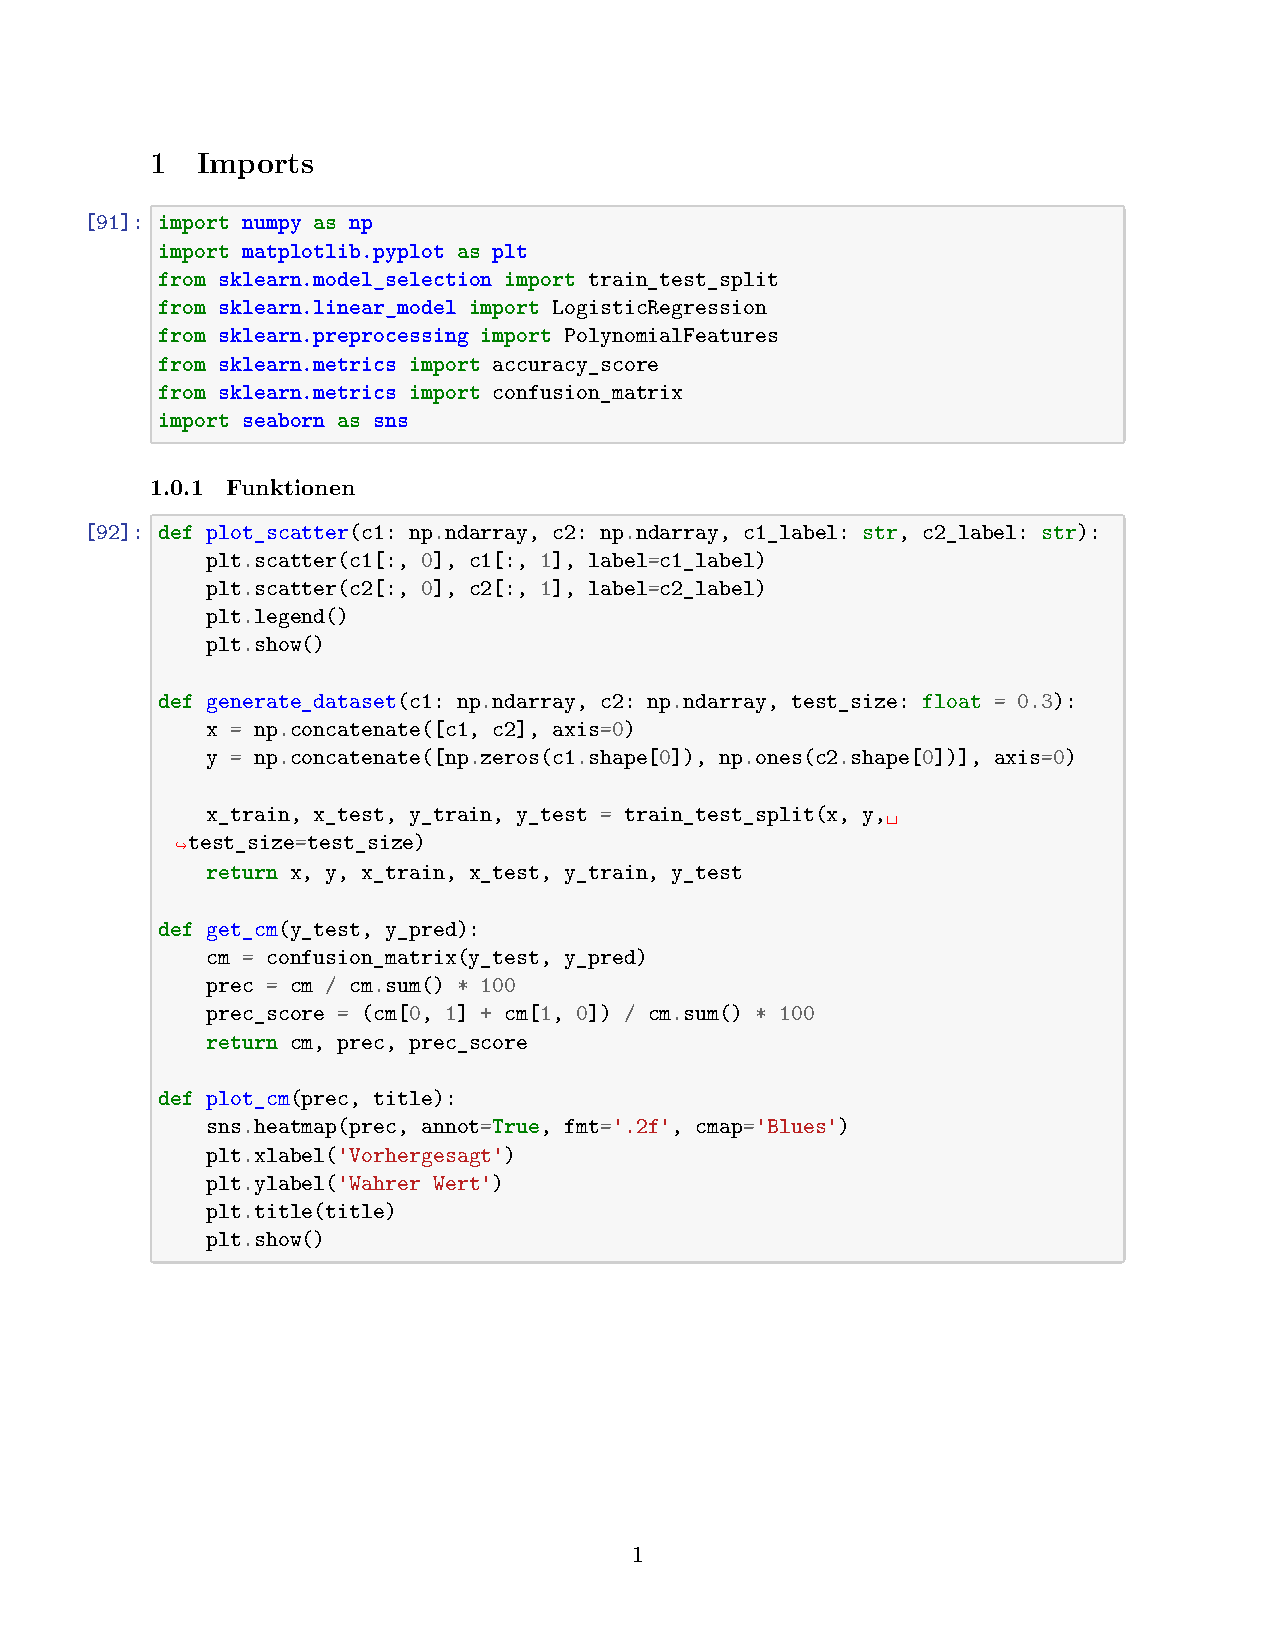
\includepdf[pages=1,pagecommand=\section*{Aufgabe 2: Polynom-Klassifikator/Aufgabe 3: Logistic-Regression-Klassifikator}]{gruppe-1-abgabe-blatt-2/aufgabe-2-3.pdf}
\includepdf[pages={2-}]{gruppe-1-abgabe-blatt-2/aufgabe-2-3.pdf}

\end{document}
